\chapter{aiVLE Gym Design}
\label{appendix:aivle-gym}
\section{Multi-agent Communication DFA}
\label{as:aivle-gym_dfa}

In this section we will define the aiVLE Gym communication DFA in a more mathematical (i.e., ``rigorous'' and detailed) fashion:

\begin{figure}[H]
    \centering
    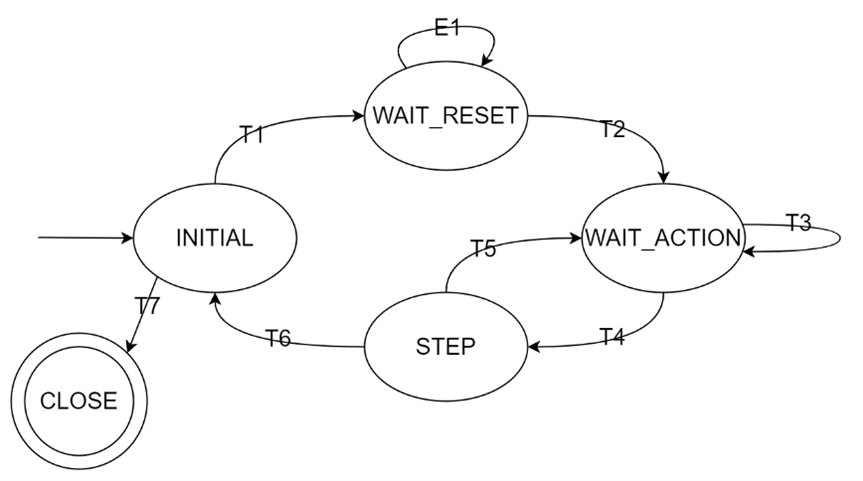
\includegraphics{images/aivle-gym-multi-dfa.png}
    \caption{aiVLE Gym Multi-agent Communication DFA}
    \label{fig:aivle-gym_dfa}
\end{figure}

\begin{enumerate}
    \item States: INITIAL, WAIT\_RESET, WAIT\_ACTION, STEP, CLOSE
    \item Initial state $q_0$: INITIAL
    \item Accept (terminal) states $F$: CLOSE
    \item Input symbols: method (e.g. reset/step/close) and other conditions
\end{enumerate}

To make this DFA a mathematically rigorous one, the domain of transition function needs to be the Cartesian product of input symbols and states. However, since there are many symbols and states involved, listing them exhaustively takes too much space. For the sake of simplicity, we omitted many self-transitioning paths - if transitioning condition is not satisfied, we assume there's a self-transition path. ``Meaningful'' transitions are described below:

\begin{itemize}
    \item T1
    \begin{itemize}
        \item condition: method is "reset"
        \item artifact: reset the underlying base Gym environment, label this agent as already reset, save this agent's router ID
    \end{itemize}
    \item E1
    \begin{itemize}
        \item condition: method is "reset" and this sender hasn't reset before
        \item artifact: label this agent as already reset, save this agent's router ID, trigger an input symbol of "E1" (This trigger is conceptually equivalent immediately checking if we can transit to the next state. Details can refer to the implementation.)
    \end{itemize}
    \item T2
    \begin{itemize}
        \item condition: input symbol of "E1", all agents are labelled as have reset
        \item artifact: send initial observation to all agents, clear reset labels, clear router ID mappings
    \end{itemize}
    \item T3
    \begin{itemize}
        \item condition: method is "step"
        \item artifact: label this agent as already stepped, save this agent's router ID, save this agent's action, trigger an input symbol of "T3"
    \end{itemize}
    \item T4
    \begin{itemize}
        \item condition: input symbol of "T3", all agents are labelled as have stepped
        \item artifact: step forward in the base environment, send observation/reward/done/info to all agents, trigger an input symbol of "T4"
    \end{itemize}
    \item T5
    \begin{itemize}
        \item condition: input symbol is "T4", some of the agents still have ongoing episode
        \item artifact: clear "have stepped" labels on all agents, clear router ID mappings
    \end{itemize}
    \item T6
    \begin{itemize}
        \item condition: input symbol is "T4", none of the agents still have ongoing episode
        \item artifact: same as T5
    \end{itemize}
    \item T7
    \begin{itemize}
        \item condition: method is "close"
        \item artifact: close the underlying environment
    \end{itemize}
\end{itemize}

By implementing this DFA carefully, the multi-agent judge environment abstract base class is capable of handling any order of incoming agent requests. Most importantly, agent-side can expect responses synchronously therefore keep all their expectations about a normal single-agent Gym environment. Note that these intricate details are not of users' (both the agent author and environment author) concern. The environment author only needs to provide implementations for the abstract methods and our library will handle the rest.